\section{Configuring ROMS for a Specific Application}
\label{Wave}
This chapter describes the parts of ROMS for which the user is
responsible when configuring it for a given application.  Section
\ref{User} describes the process in a generic fashion while
\S\ref{UpDown} and \S\ref{NEP} step through the application of SCRUM
to upwelling/downwelling and wind-driven Northeast Pacific problems,
respectively.  As distributed, ROMS is ready to run quite a few
examples, where the C preprocessor flags determine which is to be
executed.  Some of these examples are described in Haidvogel and
Beckmann \cite{Haidvogel99}. Some of them are listed here:
\begin{klist}
   \kitem{BIG\_BAD\_BASIN} This is a rectangular, flat-bottomed basin with
 double-gyre wind forcing. When run, it produces a western boundary
 current flowing into a central ``Gulf Stream''
 which goes unstable and generates eddies. The goal is to run
 adiabatically to study the homogenization of potential vorticity.
 It earned its name by taking a long time and causing difficulties
 for the spectral versions of SPEM.
%   \kitem{CANYON\_A} The canyon is a periodic channel with a steep shelf
% along one wall, where the shelf contains a steep canyon.  There is a
% periodic forcing which causes the water to oscillate along the
% channel.  The rotation and the shelf lead to non-zero mean flows,
% especially near the canyon.  Version A is homogeneous and can be
% executed with a 2-D model.  See Haidvogel and Beckmann \cite{HB97} for
% a description of the canyon problems and the gravitational adjustment
% problem.
%   \kitem{CANYON\_B} This is like Canyon A, except that it is
% stratified.
%   \kitem{DAMEE\_B}  DAMEE stands for Data Assimilation and Model
% Evaluation Experiment and is a comparison of different models of
% the North Atlantic.  Version B is a big domain
% extending from 30$^\circ$ S to 65$^\circ$ N.  Additional input files
% are required to run the DAMEE configurations.
   \kitem{GRAV\_ADJ} The gravitational adjustment problem takes place
 in a long narrow domain which is initialized with dense water at one
 end and light water at the other. At time zero, the water is released
 and it generates two propagating fronts as the light water rushes to
 fill the top and the dense water rushes to fill the bottom. This
 configuration was used to test various advection schemes.
   \kitem{OVERFLOW}   This configuration is similar to the
 GRAV\_ADJ problem, but is initialized with dense water in the shallow
part of a domain with a sloping bottom.
   \kitem{SEAMOUNT}   The seamount test was used to test the pressure
 gradient errors.  It has an idealized seamount in a periodic channel.
 See Beckmann and Haidvogel \cite{BH93} and McCalpin \cite{McCalpin94}
 for more information.
   \kitem{UPWELLING}  The upwelling/downwelling example was
 contributed by Anthony Macks and Jason Middleton \cite{Macks93}
 and consists of a periodic channel with shelves on each side.
 There is along-channel wind forcing and the Coriolis term leads
 to upwelling on one side and downwelling on the other side. If
 you run it for several days without vertical mixing, you end up with
 dense water over light water.
\end{klist}
Some input files for the ROMS examples can be found under \code{Data/ROMS}
in the ROMS distribution.

\subsection{Configuring ROMS}
\label{User}

The four main sections you need to change in ROMS are the \code{makefile}
or \code{build.bash}, an include file with \code{cpp} options, any
analytic functions, and the ascii input file. If more realistic fields
are desired, you will have to provide other input files as well, for
instance for the grid and the wind forcing.

\subsubsection{Case Name}

First, you need to decide on a name for your particular application or
configuration. This name is provided via the \code{ROMS\_APPLICATION} in
either the makefile or the build script. This name should be reasonably
short, all uppercase, with spaces converted to underscores. For example,
let's say we pick the name \code{WIKI\_TEST}. This name gets defined
during the build, so you can add code protected by \code{\#ifdef
WIKI\_TEST} as needed. This would be a good time to either copy the
makefile or the build Script to create one specific to this case prior
to editing it.

\subsubsection{ Case-specific Include File}

Each application has its own include file, included by
\code{cppdefs.h}. The name of this file is the name of your
application (\code{WIKI\_TEST} here) turned into lower case, with '.h'
appended (\code{wiki\_test.h}). The location of this file is set by
\code{MY\_HEADER\_DIR}, pointing to \code{User/Include} or some other
location of your choosing.

The complete list of options to be set prior to compilation are listed in
\S\ref{Cpp1}. Place those you need in the \code{wiki\_test.h} file. These
include algorithm choices (e.g. advection and turbulence closure schemes),
boundary conditions, output options (averages, diagnostics, stations,
floats), and application modules (biology, sediments). Each line should
be of the form:
\begin{verbatim}
        #define SOME_VAR
\end{verbatim}
Note that any undefined variable need not be mentioned.

Also note that if you copy a predefined application from
\code{ROMS/Include} as a template for your application, you must
rename it. If you don't change the name, ROMS will use the one in
\code{ROMS/Include} and your file will be ignored during the build
procedure.

\subsubsection{Functionals}

Some of the cpp Options have names beginning with \code{ANA\_}. For each one of
these, you will be expected to provide an analytic expression for the field
in question in the corresponding include file. These files
are listed in \S\ref{Funcs} and their location is determined
by \code{MY\_ANALYTICAL\_DIR}. You may chose to copy those from
\code{User/Functionals} to some new directory and place your version of
the assignments within
\begin{verbatim}
        #ifdef WIKI_TEST
	! Set weird and wonderful winds
	   :
	#endif
\end{verbatim}
This makes
it easy to search for later, if nothing else.

\subsubsection{\code{checkdefs.F}}

For each new \code{cpp} variable, it is recommended that you also
add the appropriate code to \code{checkdefs.F}, such as:
\begin{verbatim}
       #ifdef SLEET
             IF (Master) WRITE(stdout,20) 'SLEET',                      &
            &   'Sleet falling on the ice option.'
             is=lenstr(Coptions)+1
             Coptions(is:is+7)=' SLEET,'
       #endif /* ICE */
\end{verbatim}
Note that the number ``7'' on the \code{Coptions} line must be set
according to the length of the string you are adding.  In this case 7
is for `` SLEET,'', including the comma and the space.

\subsubsection{Model domain}
\label{Muddy}
One of the first things the user must decide is how many grid points
to use, and can be afforded.  There are three parameters in
\code{ocean.in} which specify the grid size and one parameter for the
number of tracers:
\begin{tabbing}
  Gnu \= Allolo \= \kill
  \> \code{Lm} \> Number of finite-difference points in $\xi$. \\
  \> \code{Mm} \> Number of finite-difference points in $\eta$. \\
  \> \code{N} \> Number of finite-difference points in the vertical. \\
  \> \code{NAT} \> Number of active tracers. \\
  \> \code{NPT} \> Number of passive tracers. \\
  \> \code{NCS} \> Number of cohesive (mud) sediment tracers. \\
  \> \code{NNS} \> Number of non-cohesive (sand) sediment tracers.
\end{tabbing}
The number of biological tracers is set in the \code{biology.in} file.
There are no constraints on these except $\code{Lm} \geq 2$, $\code{Mm}
\geq 2$, $\code{N} \geq 2$ and $\code{NAT} \geq 1$.  \code{Lm} and
\code{Mm} should be at least 3 if the domain is periodic in that
direction.

\subsubsection{$x,y$ grid}
The subroutine \code{get\_grid} or \code{ana\_grid} is called by
\code{initial} to set the grid arrays, the bathymetry, and the
Coriolis parameter.  Most of the simple test problems have their grid
information specified in \code{ana\_grid.h} in the directory
\code{ROMS/Functionals}.  More realistic problems require a NetCDF grid
file, produced by the grid generation programs described in Wilkin and
Hedstrom \cite{GRIDS}.  The variables which are read by
\code{get\_grid} are:
\begin{tabbing}
  Gnu \= \kill
  \> \code{xl, el, spherical, f, h, pm, pn, x\_rho, y\_rho,
  lon\_rho, lat\_rho, angle}.
\end{tabbing}
If the grid is curved, \code{get\_grid} will also read:
\begin{tabbing}
  Gnu \= \kill
  \> \code{dndx, dmde}.
\end{tabbing}

\subsubsection {$\xi,\eta$ grid}
Before providing initial conditions and boundary conditions, the
user must understand the model grid. The fields are laid out on an
Arakawa C grid as in Fig.\ \ref{fcgr}. The overall grid is shown in
Fig.\ \ref{fwgr}.  The thick outer line shows the position of the
model boundary. The points inside this boundary are those which are
advanced in time using the model physics. The points on the boundary
and those on the outside must be supplied by the boundary
conditions.

\begin{figure}[p]
\setlength{\unitlength}{6mm}
  \begin{picture}(25,27)(-3.0,-7)
\thicklines
  \put(3.975,4){\line(0,1){12}}
  \put(4.025,4){\line(0,1){12}}
  \put(21.975,4){\line(0,1){12}}
  \put(22.025,4){\line(0,1){12}}
  \put(4,3.975){\line(1,0){18}}
  \put(4,4.025){\line(1,0){18}}
  \put(4,15.975){\line(1,0){18}}
  \put(4,16.025){\line(1,0){18}}
\thinlines
  \multiput(7,4)(3,0){5}{\line(0,1){12}}
  \multiput(4,7)(0,3){3}{\line(1,0){18}}
\thicklines
  \put(16.3,-2.6){$\times$}
  \put(16.4,-3.5){\framebox(.2,.2){}}
  \put(16.5,-4.4){\circle{.3}}
%  \put(16.5,-5.4){\circle*{.3}}
  \put(16.9,-2.6){-- $u$ points}
  \put(16.9,-3.6){-- $v$ points}
  \put(16.9,-4.6){-- $\rho$ points}
%  \put(16.9,-5.6){-- $\psi$ points}
%  \multiput(4,4)(3,0){7}{\circle*{.3}}
%  \multiput(4,7)(3,0){7}{\circle*{.3}}
%  \multiput(4,10)(3,0){7}{\circle*{.3}}
%  \multiput(4,13)(3,0){7}{\circle*{.3}}
%  \multiput(4,16)(3,0){7}{\circle*{.3}}
  \multiput(2.5,2.5)(3,0){8}{\circle{.3}}
  \multiput(2.5,5.5)(3,0){8}{\circle{.3}}
  \multiput(2.5,8.5)(3,0){8}{\circle{.3}}
  \multiput(2.5,11.5)(3,0){8}{\circle{.3}}
  \multiput(2.5,14.5)(3,0){8}{\circle{.3}}
  \multiput(2.5,17.5)(3,0){8}{\circle{.3}}
  \multiput(2.4,3.9)(3,0){8}{\framebox(.2,.2){}}
  \multiput(2.4,6.9)(3,0){8}{\framebox(.2,.2){}}
  \multiput(2.4,9.9)(3,0){8}{\framebox(.2,.2){}}
  \multiput(2.4,12.9)(3,0){8}{\framebox(.2,.2){}}
  \multiput(2.4,15.9)(3,0){8}{\framebox(.2,.2){}}
  \multiput(3.76,2.4)(3,0){7}{$\times$}
  \multiput(3.76,5.4)(3,0){7}{$\times$}
  \multiput(3.76,8.4)(3,0){7}{$\times$}
  \multiput(3.76,11.4)(3,0){7}{$\times$}
  \multiput(3.76,14.4)(3,0){7}{$\times$}
  \multiput(3.76,17.4)(3,0){7}{$\times$}
  \put(-1,-1){\vector(1,0){10}}
  \put(-1,-1){\vector(0,1){10}}
  \put(7,-2){$\xi$}
  \put(-2,7){$\eta$}
  \put(1.5,1.2){$i=0$}
  \put(.3,2.4){$j=0$}
  \put(1.2,3.85){1}
  \put(1.2,5.35){1}
  \put(1.2,6.85){2}
  \put(1.2,8.35){2}
  \put(1.2,10.6){$\vdots$}
  \put(0.8,12.85){\code{Mm}}
  \put(0.8,14.35){\code{Mm}}
  \put(1.2,15.85){\code{M}}
  \put(1.2,17.35){\code{M}}
  \put(3.85,1.2){1}
  \put(5.35,1.2){1}
  \put(6.85,1.2){2}
  \put(8.35,1.2){2}
  \put(9.85,1.2){3}
  \put(11.35,1.2){3}
  \put(15.1,1.2){$\cdots$}
  \put(18.85,1.2){\code{Lm}}
  \put(20.35,1.2){\code{Lm}}
  \put(21.85,1.2){\code{L}}
  \put(23.35,1.2){\code{L}}
  \end{picture}
  \caption{The whole grid. Note that there are \code{Lm} by \code{Mm}
  interior computational points. The points on the thick outer line and
  those outside it are provided by the boundary conditions.}
\label{fwgr}
\end{figure}

The three-dimensional model fields are carried in four-dimensional
arrays, where the fourth array index refers to one of three
time levels. The tracers have a fifth array index tells which
tracer is being referred to.
For instance, $\code{itemp}=1$ refers to
potential temperature while $\code{isalt}=2$ refers to salinity.  The
integers $i$, $j$, and $k$ are used throughout the model to index
the three spatial dimensions:
\begin{tabbing}
Gnus \= Gnus \= \kill
   \>$i$ \>Index variable for the $\xi$-direction. \\
   \>$j$ \>Index variable for the $\eta$-direction. \\
   \>$k$ \>Index variable for the $\sigma$-direction.  $k = 1$
   refers to the bottom \\
biggnu \= \kill
   \>while $k = \code{N}$ refers to the surface.
\end{tabbing}

%The range of $\xi$ is 1 to \code{L} and the range of $\eta$ is 1 to
%\code{M}.  Therefore $i$ and $\xi$ are the same at $\psi$
%points, as are $j$ and $\eta$.  (This matters in the floats---Dale and
%I disagreed on how this should be and then Dale later changed to my
%point of view after I had recoded things to match his).

\subsubsection{Initial conditions}
The initial values for the model fields are provided by either
\code{ana\_initial} or \code{get\_state}.  \code{get\_state} is
also used to read a restart file if the model is being restarted from a
previous run.

Also in \code{initial}, \code{rho\_eos} is called to initialize
the density field. \code{rho\_eos} also computes \code{rhoA},
the vertically averaged density, and \code{rhoS}, the density
perturbation. Both \code{rhoA} and \code{rhoS} are used in the barotropic
pressure gradient.

%The tracer climatology fields also require appropriate values if they
%are to be used, and are provided by \code{ana\_tclima} or
%\code{get\_tclima}. Likewise, the surface height climatology is read by
%\code{get\_ssh} or provided by \code{ana\_ssh}.

\subsubsection{Equation of state}
The equation of state is defined in the subroutine \code{rho\_eos}.  Two
versions are provided in ROMS: a nonlinear $\rho =
\rho(T,S,z)$ from Jackett and McDougall \cite{Jackett} and a linear
$\rho(T,S)$.  The linear form is
$$
      \rho = \code{R0} - \code{Tcoef} \cdot (T-T0) +
      \code{Scoef} \cdot (S-S0)
$$
or
$$
     \rho = \code{R0} + \code{Tcoef} \cdot (T-T0),
$$
depending on whether or not
\code{SALINITY} is defined.  Specify which equation of state you
would like to use with the \code{NONLIN\_EOS} C preprocessor flag your
application include file. The linear coefficients \code{R0}, \code{T0},
\code{Tcoef}, \code{S0}, and \code{Scoef} are set in \code{ocean.in}. Note
that we are computing {\em in situ} density from potential temperature and
salinity. Some of the vertical mixing schemes require potential density
and some other terms, which are computed by \code{rho\_eos} as well.

\subsubsection{Boundary conditions}
\label{Bcs}
The horizontal boundary conditions are provided by the subroutines
in \code{u3dbc\_im}, \code{v3dbc\_im}, \code{u2dbc\_im}, \code{v2dbc\_im},
\code{t3dbc\_im}, and \code{zetabc}.  They are called every timestep
and provide the boundary values for the fields $u, v, \overline{u},
\overline{v}$, all tracers, and $\zeta$, respectively. They are currently
configured for a closed basin, a periodic channel, a doubly periodic
domain or an open domain with various radiation conditions. Each side is
controlled independently with \code{WEST} being the \code{i=1} boundary,
\code{EAST} being the \code{i=L} boundary, \code{SOUTH} being the \code{j=1}
boundary, and \code{NORTH} being the \code{j=M} boundary. These choices are
made via the \code{cpp} options in your include file.

\subsubsection{Model forcing}
\label{Mforce}
\noindent {\bf(a) Winds and thermal fluxes}

There are two different ways to apply a wind forcing: as a surface
momentum flux in the vertical viscosity term, or as a body force over
the upper water column.  In the past, our vertical resolution was
relatively coarse and the vertical viscosity would have to have been
unreasonably large for us to resolve the surface Ekman layer.  If that
is your situation, define \code{BODYFORCE} in \code{cppdefs.h} and
provide a value for \code{levsfrc} in \code{scrum.in}.  The forcing is
applied over the levels from \code{levsfrc} to \code{N}.  The above
caution about vertical resolution also applies to the surface fluxes of
$T$ and $S$, although \code{BODYFORCE} only refers to wind stress, not
the surface tracer fluxes.
%In addition, if you have vertical diffusion
%of tracers and no surface fluxes, you will erode the vertical
%stratification unless \code{CLIMAT\_TS\_MIXV} is defined.

More recently, we have been setting the vertical $s$-coordinate
parameters to retain some resolution near the surface and to apply the
fluxes as boundary conditions to the vertical viscosity/diffusivity.
In either case, the surface and bottom fluxes are either defined
analytically or read from the forcing file.  You must either edit the
appropriate parts of \code{analytical.F} or create a NetCDF forcing
file in the format expected by \code{get\_smflux}, \code{get\_stflux}
and their friends.  Note that it is quite common to put the wind
stress into the forcing file while having an analytic bottom stress.

\smallskip
\noindent {\bf(b) Climatology}

One way to force the model is via a nudging to the tracer climatologies.
This was is used in the North Atlantic simulations in sponge layers
along the northern and southern boundaries.  Set the climatologies
in \code{ana\_tclima} or in a file read by \code{get\_tclima}, set
\code{NUDGING} in \code{cppdefs.h} and also
set the array \code{nudgcof} in \code{set\_nudgcof.F}.


\subsubsection{\code{scrum.in}}
SCRUM expects to read a number of variables on standard in.  It is
easiest to prepare an input file and then run SCRUM as:
\begin{verbatim}
       scrum < scrum.in > scrum.out &
\end{verbatim}
The input is organized as pairs of lines, the first with a number and
then some text which is ignored, the second with the values for the
set of variables for which the first line provides the key.  The pairs
of lines can be in any order but are usually sorted numerically.  The
number 99 signals the end of these pairs and the rest of the input file
contains comments for the user.  The input pairs are as follows:
\begin{klist}
   \kitem{\qquad 1} Time-stepping parameters.
     \begin{klist}
       \kitem{ntimes}    Number of timesteps to evolve the 3-D
       equations in the current run.  This is actually the total
     number, including any previous segments of the same run.  For
     instance, if you already did a three-month run and wish to
     continue for another three months, set \code{ntimes} to the
     number of steps needed for six months.  If you don't like this
     and would prefer to have the behavior of the SPEM variable
     \code{ntmes}, modify \code{main.F} so that:
     \begin{verbatim}
        do iic=ntstart,ntimes
     \end{verbatim}
     becomes
     \begin{verbatim}
        do iic=ntstart,ntimes-1+ntstart
     \end{verbatim}
       \kitem{dt}        Timestep in seconds for the 3-D equations.
       \kitem{ndtfast}   Number of timesteps for the 2-D equations
     to be executed each \code{dt}.
     \end{klist}
   \kitem{\qquad 2}   Input/Output parameters.  SCRUM has several
   possible output files.  The output files
   include a restart file, a history file, an averages file, and a
   station file.  The restart file often contains only two records with
   the older record being overwritten during the next write.  The
   history file can contain a subset of the restart fields, for
   instance just the surface elevation and the surface temperature.
   The averages file contains time-averages of the model fields, for
   instance montly means, or yearly means, depending on \code{navg}.
   The station file contains timeseries for specified points, possibly
   quite frequently since each record is small.
     \begin{klist}
       \kitem{nrrec}     Record number of the restart file to read
     as the initial conditions.
       \kitem{nrreci}    Record number of the ice restart file to read
     as the initial conditions (coupled ice model only).
       \kitem{nrst}      Number of timesteps between writing of
     restart fields.
       \kitem{nwrt}      Number of timesteps between writing fields
     into the history file.
       \kitem{ntsavg}    Starting timestep for the accumulation of
     output time-averaged data.  For instance, you might want to average
     over the last day of a thirty-day run.
       \kitem{navg}      Number of timesteps between writing
     time-averaged data into the averages file.
       \kitem{nsta}      Number of timesteps between writing data into
     stations file.
       \kitem{ninfo}     Number of timesteps between printing a single
     line of diagnostic information to the standard output.
       \kitem{ldefhis}   Logical switch used to create the history
     file.  If \code{.true.}, a new history file is created.  If
     \code{.false.} and $\code{nlev} > 0$, data is appended to an
     existing history file.
       \kitem{lcycle}    Logical flag used to recycle time records in
     the restart file. If \code{.true.}, only the latest two restart
     time records are retained.  If \code{.false.}, all restart
     fields are saved every \code{nrst} timesteps without recycling.
     \end{klist}
   \kitem{\qquad 3}   Laplacian horizontal mixing of tracers.
     \begin{klist}
       \kitem{tnu2}     Constant mixing
     coefficient for the horizontal Laplacian diffusion of each tracer.
     A value is expected for each of the \code{NT} tracers.
     \end{klist}
   \kitem{\qquad 4}   Biharmonic horizontal mixing of tracers.
     \begin{klist}
       \kitem{tnu4}     Constant mixing
     coefficient for the horizontal biharmonic diffusion of each tracer.
     A value is expected for each of the \code{NT} tracers.
     \end{klist}
   \kitem{\qquad 5}   Isopycnal thicknesses.
     \begin{klist}
       \kitem{Kdiff} Isopycnal mixing thickness diffusivity for
     each tracer variable. A value is expected for each of the
     \code{NT} tracers. These isopycnal thicknesses are used when the
     Gent/McWilliams isopycnic mixing is activated (not currently
     implimented).
     \end{klist}
   \kitem{\qquad 6}   Horizontal viscosity coefficients.
     \begin{klist}
       \kitem{uvnu2}    Constant mixing coefficient for the horizontal
     Laplacian viscosity.
       \kitem{uvnu4}    Constant mixing coefficient for the horizontal
     biharmonic viscosity.
     \end{klist}
   \kitem{\qquad 7}   Vertical mixing coefficients for tracers.
     \begin{klist}
       \kitem{akt\_bak}  Background vertical mixing coefficient
     for the tracers.
     A value is expected for each of the \code{NT} tracers.
     \end{klist}
   \kitem{\qquad 8}   Vertical mixing coefficient for momentum.
     \begin{klist}
       \kitem{akv\_bak}  Background vertical mixing coefficient 
     for momentum.
     \end{klist}
   \kitem{\qquad 9}   Mellor-Yamada Level 2.5 parameters.
     \begin{klist}
       \kitem{akq\_bak}  Background vertical mixing coefficient
     for turbulent kinetic energy.
       \kitem{q2nu2}    Constant mixing coefficient for the horizontal
     Laplacian diffusion of turbulent kinetic energy.
       \kitem{q2nu4}    Constant mixing coefficient for the horizontal
     biharmonic diffusion of turbulent kinetic energy.
     \end{klist}
   \kitem{\qquad 10}   Bottom drag coefficients.
     \begin{klist}
       \kitem{rdrg}     Linear bottom drag coefficient.
       \kitem{rdrg2}    Quadratic bottom drag coefficient.
       \kitem{Zo}       Bottom roughness.
     \end{klist}
   \kitem{\qquad 11}  Various parameters.
     \begin{klist}
       \kitem{nmix\_en}  Number of timesteps between computations of
     isopycnal slopes used in the rotated mixing tensor.
       \kitem{adv\_ord}  Order of advection scheme when using
     Smolarkiewicz advection.  A value of $\code{adv\_ord}=2$ is
     recommended to suppress the diffusive nature of the ``upwind''
     scheme.  A value of $\code{adv\_ord}=1$
     will yield the standard ``upwind'' advection.
       \kitem{levsfrc}  Deepest level to apply surface momentum
     stresses as a body force.
            Used when the C-preprocessor option BODYFORCE is defined.
       \kitem{levbfrc}  Shallowest level to apply bottom momemtum
    stresses as a body force.
            Used when the C-preprocessor option BODYFORCE is defined.
     \end{klist}
   \kitem{\qquad 12}  Vertical $s$-coordinates parameters.
     \begin{klist}
       \kitem{theta\_s}  $s$-coordinate surface control parameter,
     [$0 < \code{theta\_s} < 20$].
       \kitem{theta\_b}  $s$-coordinate bottom  control parameter,
     [$0 < \code{theta\_b} < 1$].
       \kitem{Tcline}   Width of the surface or bottom boundary layer
     in which higher vertical resolution is required during stretching.

       {\bf WARNING}: Users need to experiment with these parameters. We
                     have found out that the model goes unstable with
                     high values of \code{theta\_s}.  With steep and
                     very tall topography, it is recommended that you
                     use $\code{theta\_s} \leq 3.0$.
     \end{klist}
   \kitem{\qquad 13}  Mean Density and time stamp.
     \begin{klist}
       \kitem{rho0}     Mean density used in the Boussinesq
     approximation.
       \kitem{dstart}   Time stamp assigned to model initialization
     (days).  Usually a Calendar linear coordinate, like modified
     Julian day. For example:
     \begin{quote}
               $\code{dstart}=10200$   corresponds to   May 1, 1996
     \end{quote}
     It is called modified Julian day because an offset of 2440000
     needs to be added.
       \kitem{rnudg}    Time scale (days) of nudging towards
     climatology at the interior and at the boundaries.
     \end{klist}
   \kitem{\qquad 14}  Nudging/relaxation time scales.
     \begin{klist}
       \kitem{Znudg}    Time scale (days) of nudging towards
     sea surface height climatology.
       \kitem{M2nudg}    Time scale (days) of nudging towards
     2-D momenum climatology.
       \kitem{M3nudg}    Time scale (days) of nudging towards
     3-D momenum climatology.
       \kitem{Tnudg}    Time scale (days) of nudging towards
     tracer climatology.
     A value is expected for each of the \code{NT} tracers.
     \end{klist}
   \kitem{\qquad 15}  Linear equation of state parameters.
     \begin{klist}
       \kitem{R0}       Background density value used in
    the linear equation of state.
       \kitem{T0}       Background potential temperature constant used
    in \code{analytical.F}.
       \kitem{S0}       Background salinity constant used
    in \code{analytical.F}.
       \kitem{Tcoef}    Thermal expansion coefficient in the linear
    equation of state.
       \kitem{Scoef}    Saline contraction coefficient in the linear
    equation of state.
     \end{klist}
   \kitem{\qquad 16}  Slipperiness parameters.
     \begin{klist}
       \kitem{gamma2}   Slipperiness variable, either 1.0 (free
     slip) or $-1.0$ (no slip).
       \kitem{wall1}    Logical switch for side 1 ($i=1$), \code{.true.}
     if it is a wall, \code{.false.} if it is open.
       \kitem{wall2}    Logical switch for side 2 ($j=1$), \code{.true.}
     if it is a wall, \code{.false.} if it is open.
       \kitem{wall3}    Logical switch for side 3 ($i=\code{L}$),
     \code{.true.}
     if it is a wall, \code{.false.} if it is open.
       \kitem{wall4}    Logical switch for side 4 ($j=\code{M}$),
     \code{.true.}
     if it is a wall, \code{.false.} if it is open.
     \end{klist}
   \kitem{\qquad 17}  Logical switches to activate the writing of fields
  associated with the momentum equations into the NetCDF history file:
     \begin{klist}
       \kitem{wrtU}     Write out 3-D $u$-velocity component.
       \kitem{wrtV}     Write out 3-D $v$-velocity component.
       \kitem{wrtW}     Write out 3-D $w$-velocity component.
       \kitem{wrtO}     Write out 3-D $\Omega$ vertical velocity.
       \kitem{wrtUBAR}  Write out 2-D $u$-velocity component.
       \kitem{wrtVBAR}  Write out 2-D $v$-velocity component.
       \kitem{wrtZ}     Write out free-surface.
     \end{klist}
   \kitem{\qquad 18}  Logical switches to activate the writing of
     fields associated with the tracer equations into the NetCDF history
     file.  A value is expected for each of the \code{NT} tracers.
     \begin{klist}
       \kitem{wrtT}     Write out tracer type variables: potential
    temperature, salinity, etc.
     \end{klist}
   \kitem{\qquad 19}  Logical switches to activate the writing of
   other fields into the NetCDF history file:
     \begin{klist}
       \kitem{wrtRHO}   Write out density anomaly.
       \kitem{wrtAKV}   Write out vertical viscosity coefficient.
       \kitem{wrtAKT}   Write out vertical diffusion coefficient for
     temperature.
       \kitem{wrtAKS}   Write out vertical diffusion coefficient for
     salinity.
       \kitem{wrtHBL}   Write out depth of the planetary boundary layer.
     \end{klist}
   \kitem{\qquad 20}  Number and Levels to output:
     \begin{klist}
       \kitem{nlev}  Number of levels to write out to the history
    file for each activated 3-D field. If $\code{nlev}<0$, all
    model levels are written out. IF $\code{nlev}=0$, the history
    file will not be created.
       \kitem{lev}  If $\code{nlev}>0$, levels to write out to the
    history file.  \code{nlev} values are expected:
\[
                       1 \leq \code{lev}(1:\code{nlev}) \leq \code{N}
\]
            Enter values in ascending numerical order.
     \end{klist}
   \kitem{\qquad 21}  String with a maximum of eighty characters.
     \begin{klist}
       \kitem{title}    Title of the model run.
     \end{klist}
   \kitem{\qquad 22}  String with a maximum of eighty characters.
     \begin{klist}
       \kitem{rstname}  Output restart file name (NetCDF).
     \end{klist}
   \kitem{\qquad 23}  String with a maximum of eighty characters.
     \begin{klist}
       \kitem{hisname}  Output history file name (NetCDF).
     \end{klist}
   \kitem{\qquad 24}  String with a maximum of eighty characters.
     \begin{klist}
       \kitem{avgname}  Name of the file for the averaged model fields
     (NetCDF).
     \end{klist}
   \kitem{\qquad 25}  String with a maximum of eighty characters.
     \begin{klist}
       \kitem{staname}  Name of the file for the station output
    (NetCDF).
     \end{klist}
   \kitem{\qquad 26}  String with a maximum of eighty characters.
     \begin{klist}
       \kitem{fltname}  Name of the file containing the float output
     (NetCDF). Not implemented yet.
     \end{klist}
   \kitem{\qquad 27}  String with a maximum of eighty characters.
     \begin{klist}
       \kitem{grdname}  Name of the file containing the grid data
     (NetCDF).
     \end{klist}
   \kitem{\qquad 28}  String with a maximum of eighty characters.
     \begin{klist}
       \kitem{ininame}  Name of the file containing the initial
     conditions.  It can be a SCRUM restart file (NetCDF).
     \end{klist}
   \kitem{\qquad 29}  String with a maximum of eighty characters.
     \begin{klist}
       \kitem{frcname}  Name of the file containing the forcing fields
     (NetCDF).
     \end{klist}
   \kitem{\qquad 30}  String with a maximum of eighty characters.
     \begin{klist}
       \kitem{clmname}  Name of the file containing the climatology
     fields (NetCDF).
     \end{klist}
   \kitem{\qquad 31}  String with a maximum of eighty characters.
     \begin{klist}
       \kitem{assname}  Name of the file containing the assimilation
     fields (NetCDF).
     \end{klist}
   \kitem{\qquad 32}  String with a maximum of eighty characters.
     \begin{klist}
       \kitem{aparnam}  Name of the file containing the assimilation
     parameters (ASCII).
     \end{klist}
   \kitem{\qquad 33}  String with a maximum of eighty characters.
     \begin{klist}
       \kitem{sposnam}  Name of the file containing the stations
     positions (ASCII).
     \end{klist}
   \kitem{\qquad 34}  String with a maximum of eighty characters.
     \begin{klist}
       \kitem{fposnam}  Name of the file containing the initial drifter
     positions (ASCII).
     \end{klist}
   \kitem{\qquad 35}  String with a maximum of eighty characters.
     \begin{klist}
       \kitem{iininame}  Name of the ice input file (coupled ice model
       only).
     \end{klist}
   \kitem{\qquad 36}  String with a maximum of eighty characters.
     \begin{klist}
       \kitem{irstnam}  Name of the ice restart file (coupled ice model
       only).
     \end{klist}
   \kitem{\qquad 37}  String with a maximum of eighty characters.
     \begin{klist}
       \kitem{ihisnam}   Name of the ice history file (coupled ice
       model only).
     \end{klist}
   \kitem{\qquad 38}  String with a maximum of eighty characters.
     \begin{klist}
       \kitem{iavgnam}   Name of the ice averages file (coupled ice
       model only).
     \end{klist}
   \kitem{\qquad 39}  String with a maximum of eighty characters.
     \begin{klist}
       \kitem{usrname}  User's generic input file name.
     \end{klist}
\end{klist}
An example input file without the trailing comments is:
\begin{verbatim}
1    NTIMES,     DT (s),    NDTFAST
      1800       240.d0       20 
2    NRREC,   NRST,   NWRT,  NTSAVG,   NAVG,   NSTA,  NINFO,  LDEFHIS,  LCYCLE
       0       360     360      1       360      1      1        T        T
3    TNU2[1:NT]  (m^2/s)
     5.d0        5.d0     
4    TNU4[1:NT]  (m^4/s)
      1.0d+07     1.0d+07
5    Kdiff[1:NT] (m2/s)
       0.d0      0.d0
6    UVNU2 (m^2/s),   UVNU4 (m^4/s)
      10.d0           0.d0
7    AKT_BAK[1:NT] (m^2/s)
     1.0d-5    1.0d-5
8    AKV_BAK (m^2/s)
     1.0d-4
9    AKQ_BAK (m^2/s)  Q2NU2 (m^2/s),   Q2NU4 (m^4/s)
     1.0d-4             20.d0           1.0d+07
10   RDRG (m/s),      RDRG2,      Zo (m)
     4.5E-04          0.d0         0.d0
11   NMIX_EN,    ADV_ORD,   LEVSFRC,   LEVBFRC
        1           2          1          1
12   THETA_S,   THETA_B,    TCLINE (m)
      3.d0      0.d0         50.d0
13   RHO0 (Kg/m^3),  DSTART (days)
     1025.d0         0.d0
14   ZNUDG (days), M2NUDG (days), M3NUDG(days), TNUDG[1:NT] (days)
     0.d0           0.d0           0.d0           0.d0    0.d0
15   R0 (Kg/m^3)  T0 (deg C),  S0 (PSU),     TCOEF,      SCOEF
     1026.9524      10.d0        35.d0     -1.67e-04   7.62e-04
16   GAMMA2,  WALL1,  WALL2,  WALL3,   WALL4
       1.d0     T       F       F       F 
17   wrtU,    wrtV,   wrtW,   wrtO,   wrtUBAR,  wrtVBAR,  wrtZ
       T        T       T       F       F         F         T
18   wrtT(1:NT)    (temperature, salinity, etc.)
       T        T
19   wrtRHO,  wrtAKV, wrtAKT, wrtAKS, wrtHBL
       F        F       F       F       F
20   NLEV,  LEV(1:NLEV)  in ascending order (if NLEV<0, all levels are saved)
      -1     1 3 5
21   TITLE (a80)
Scrum 4.0
22   RSTNAME (a80): SCRUM output restart file name, if any.
scrum_rst.nc
23   HISNAME (a80): SCRUM output history file name, if any.
scrum_his.nc
24   AVGNAME (a80): SCRUM output averages file name, if any.
scrum_avg.nc
25   STANAME (a80): SCRUM output stations file name, if any.
scrum_sta.nc
26   FLTNAME (a80): SCRUM output floats file name, if any.
scrum_flt.nc
27   GRDNAME (a80): SCRUM input grid file name, if any.
scrum_grd.nc
28   ININAME (a80): SCRUM input initial conditions file name, if any.
scrum_ini.nc
29   FRCNAME (a80): SCRUM input forcing fields file name, if any.
scrum_frc.nc
30   CLMNAME (a80): SCRUM input climatology fields file name, if any.
scrum_clm.nc
31   ASSNAME (a80): SCRUM input assimilation fields file name, if any.
scrum_ass.nc
32   APARNAM (a80): SCRUM input assimilation parameters file name, if any.
assimilation.dat
33   SPOSNAM (a80): SCRUM input station positions file name, if any.
stations.dat
34   FPOSNAM (a80): SCRUM input initial floats positions file name, if any.
floats.dat
35   USRNAME (a80): USER's input/output generic file name, if any.
/dev/null
99   END of input data
\end{verbatim}

\subsubsection{User variables and subroutines}
\label{Store}
It is possible for the user to add new variables and common blocks
appropriate to a given application.  It is also possible to add
new subroutines, for instance to read in river inflow data.  If
you create new source files they will have to be added to the
\code{Makefile} or the \code{Imakefile} (see \S\ref{Imake}).  Also,
any new \code{\#include} statements will have to
be listed in the \code{Makefile} dependencies.  The simplest way
to add them is to run \code{make depend}.

\subsection{Upwelling/Downwelling Example}
\label{UpDown}
One application for which SCRUM has been configured is a wind-driven
upwelling and downwelling example, described in Macks and Middleton
\cite{Macks93}.  There is a shelf on each wall of a periodic channel
and an along-channel wind forcing, which drives upwelling at one wall
and downwelling at the other.  This problem depends on the Ekman layer,
so a surface stress is used with vertical viscosity.  The Ekman depth
is estimated to be 9 $m$ if $A_v = 0.01 m^2 / s$, so the vertical grid
spacing must resolve this.  The maximum depth is 150 $m$ and our choice
of the vertical grid parameters leads to a surface $\Delta z$ of 4.0
$m$.

\subsubsection{\code{cppdefs.h}}
The C preprocessor variable \code{UPWELLING} has been introduced to
make sure that we can \code{\#define UPWELLING} and have a consistent
upwelling configuration of the model.  This is done in part
within \code{cppdefs.h} by
\begin{verbatim}
        #ifdef UPWELLING
        #define UV_ADV
        #undef  UV_VIS2 
        #define UV_PRS
        #define UV_COR
        #define TS_ADV
        #undef  TS_DIF2
        #undef        NONLIN_EOS
        #undef        SALINITY
        #undef        CURVGRID
        #define       EW_PERIODIC
        #undef        NS_PERIODIC
        #define TIME_AVG
        #undef  BODYFORCE
        #define ANA_GRID
        #define ANA_INITIAL
        #define ANA_MEANRHO
        #define ANA_SMFLUX
        #define ANA_STFLUX
        #define ANA_SSFLUX
        #define ANA_BTFLUX
        #define ANA_BSFLUX
        #define ANA_VMIX
        #endif  /* UPWELLING */
\end{verbatim}
Here we have declared that we want a periodic channel but no masking.
There is neither salinity nor climatology.  The momentum equations have
the Coriolis and pressure gradients, but no horizontal viscosity.  The
only term in the tracer equation is the advection.

\subsubsection{Model domain}
The flow does not vary in $x$, so \code{L} can be small.
Set the values for \code{L}, \code{M}, \code{N} and \code{NT} in
\code{param.h}:
\begin{tabbing}
  Gnus Armadillos Pelicans \= \kill
  \> \code{L} = 42 \\
  \> \code{M} = 81 \\
  \> \code{N} = 16 \\
  \> \code{NT} = 2.
\end{tabbing}

\subsubsection{\code{ana\_grid}}
For this geometry one has a choice of using the grid-generation
programs described in Wilkin and Hedstrom \cite{GRIDS}, or of
using \code{ana\_grid} to create the grid analytically.
The \code{ana\_grid} subroutine in \code{analytical.F} was
modified to produce a bathymetry with a shelf on both walls of the
channel when \code{UPWELLING} is defined.  The fluid depth ranges from
27 $m$ on the shelves to 150 $m$ in the center of the channel.
The horizontal grid spacing is uniform at 1 $km$ and the
Coriolis parameter $f$ is set to a constant value suitable for
Sydney, Australia.

\subsubsection{Initial conditions and the equation of state}
We would like the initial conditions to be a motionless fluid with an
exponential stratification.  \code{ana\_initial} is configured
accordingly.

The stratification can be provided by either $T$ or $S$, or by both
$T$ and $S$.  For
simplicity we will only have an active temperature field and we will
use the linear equation of state by setting \code{NONLIN\_EOS} to
\code{\#undef} in \code{rhsdefs.h}.  We want the density to be 26.35 at
the bottom and 24.22 at the top with an e-folding scale of 50 meters.
The initial temperature is set to $14 + 8\mbox{e}^{z/50}$ in
\code{ana\_initial}.  The linear equation of state parameters are set
in \code{scrum.in}.

Since density does not depend on salinity, we have a choice of how to
handle the second tracer.  We can either use it as a passive tracer or
not timestep on it at all by setting $\code{NT}=1$.  We will use
it as a passive tracer and initialize it to be a
function of $y$.

We have set \code{ana\_meanRHO} to the desired initial density field.
The climatology fields are not used and need not be initialized.

\subsubsection{Boundary conditions}
The periodic channel options have already been chosen in
\code{cppdefs.h}.  We do not have to do anything else.

\subsubsection{Model forcing}
In this problem we want to resolve the
surface Ekman layer and to use a surface wind stress rather than a body
force.  We want the amplitude of the wind to ramp up with time so we
modify \code{ana\_smflux} accordingly.
The wind will build to an amplitude of 0.1 Pascals / $\rho_o$,
or $10^{-4} m^2 s^{-2}$.

We need to edit \code{ana\_vmix} to make sure that the
vertical viscosity \code{Akv} is set to the value we want.  This
must be large at the surface ($10^{-2} m^2 s^{-1}$) to create a thick
Ekman layer, but has been chosen to decrease with depth.  We also need
to check that \code{ana\_sbflux}, \code{ana\_stflux}, etc.\ are
set correctly.

\subsubsection{scrum.in}
The model has been set up to run for one day with an internal timestep
of 120 $s$ and an external timestep of 12 $s$.  We will write history
and restart records every 1/4 day.  The value of the linear bottom
friction coefficient \code{rdrg} is set to $4.5 \times 10^{-4}$ and the
channel walls are set to be free-slip.

\subsubsection{Output}
The model writes some information to standard out, after setting
\code{ninfo} to 72:
\begin{verbatim}

 SCRUM input parameters:

       720  ntimes      Number of timesteps to evolve 3-D equations.
    120.00  dt          Timestep size (s) for 3-D equations.
        10  ndffast     Number of timesteps for 2-D equations between each DT.
         0  nrrec       Number of restart records to read from disk.
       180  nrst        Number of timesteps between storage of restart fields.
       180  nwrt        Number of timesteps between writing fields into
                        history file.
        72  ninfo       Number of timesteps between print of information
                        to standard output.
         T  ldefhis     Switch to create a new history NetCDF file.
         T  lcycle      Switch to recycle time-records in restart NetCDF file.
 0.000E+00  tnu2(1)     Horizontal, Laplacian mixing coefficient (m^2/s)
                        for tracer 1.
 0.000E+00  tnu2(2)     Horizontal, Laplacian mixing coefficient (m^2/s)
                        for tracer 2.
 0.000E+00  uvnu2       Horizontal, Laplacian mixing coefficient (m^2/s)
                        for momentum.
 0.000E+00  Akt_bak(1)  Background vertical mixing coefficient (m^2/s)
                        for tracer 1.
 0.000E+00  Akt_bak(2)  Background vertical mixing coefficient (m^2/s)
                        for tracer 2.
 1.000E-05  Akv_back    Background vertical mixing coefficient (m^2/s)
                        for momentum.
 4.500E-04  rdrg        Linear bottom drag coefficient (m/s).
 0.000E+00  rdrg2       Quadratic bottom drag coefficient.
 3.000E+00  theta_s     S-coordinate surface control parameter.
 0.000E+00  theta_b     S-coordinate bottom  control parameter.
   50.0000  Tcline      S-coordinate surface/bottom layer width (m) used
                        in vertical coordinate stretching.
 1000.0000  rho0        Mean density (kg/m^3) used in Boussinesq approximation.
    0.0000  dstart      Time stamp assigned to model initialization (days).
 0.000E+00  Znudg       Nudging/relaxation inverse time scale (1/days)
                        for free-surface.
 0.000E+00  M2nudg      Nudging/relaxation inverse time scale (1/days)
                        for 2D momentum.
 0.000E+00  M3nudg      Nudging/relaxation inverse time scale (1/days)
                        for 3D momentum.
 0.000E+00  Tnudg(1)    Nudging/relaxation inverse time scale (1/days)
                        for tracer 1.
 0.000E+00  Tnudg(2)    Nudging/relaxation inverse time scale (1/days)
                        for tracer 2.
    0.0000  T0          Background potential temperature (Celsius) constant.
    0.0000  S0          Background salinity (PSU) constant.
   30.3795  R0          Background density (kg/m^3) used in linear Equation
                        of State.
-2.800E-01  Tcoef       Thermal expansion coefficient (1/Celsius).
 0.000E+00  Scoef       Saline contraction coefficient (1/PSU).
      1.00  gamma2      Slipperiness variable: free-slip (1.0) or 
                                               no-slip (-1.0).
         F  wall1       Boundary for side 1 (i=1): wall/open (T/F).
         T  wall2       Boundary for side 2 (j=1): wall/open (T/F).
         F  wall3       Boundary for side 3 (i=L): wall/open (T/F).
         T  wall4       Boundary for side 4 (j=M): wall/open (T/F).
         T  wrtU        Write out 3D U-momentum component (T/F).
         T  wrtV        Write out 3D V-momentum component (T/F).
         T  wrtW        Write out W-momentum component (T/F).
         T  wrtO        Write out omega vertical velocity (T/F).
         T  wrtUBAR     Write out 2D U-momentum component (T/F).
         T  wrtVBAR     Write out 2D V-momentum component (T/F).
         T  wrtZ        Write out free-surface (T/F).
         T  wrtT(1)     Write out tracer 1 (T/F).
         T  wrtT(2)     Write out tracer 2 (T/F).
         T  wrtRHO      Write out density anomaly (T/F).
         F  wrtAKV      Write out vertical viscosity coefficient (T/F).
         F  wrtAKT      Write out vertical T-diffusion coefficient (T/F).
         F  wrtAKS      Write out vertical S-diffusion coefficient (T/F).
        16  Nlev        Number of levels to write out.
            Lev         Levels to write out:
                        01 02 03 04 05 06 07 08 09 10 11 12 13 14 15 16

Upwelling/Downwelling Example on a Periodic Double Shelf Channel
       


 Output/Input Files:

            Output Restart File:  scrum_rst.nc
            Output History File:  scrum_his.nc
         Input/Output USER File:  /dev/null

 Activated C-preprocessing Options:

  ANA_BSFLUX       Analytical kinematic bottom salt flux.
  ANA_BTFLUX       Analytical kinematic bottom heat flux.
  ANA_GRID         Analytical grid set-up.
  ANA_INITIAL      Analytical initial conditions.
  ANA_MEANRHO      Analytical mean density anomaly.
  ANA_SMFLUX       Analytical kinematic surface momentum flux.
  ANA_SSFLUX       Analytical kinematic freshwater (E-P) flux.
  ANA_STFLUX       Analytical kinematic surface heat flux.
  ANA_VMIX         Analytical vertical mixing coefficients.
  DBLEPREC         Double precision arithmetic.
  EW_PERIODIC      East-West periodic boundaries.
  MIX_GP_TS        Mixing of tracers along geopotential surfaces.
  MIX_GP_UV        Mixing of momentum along geopotential surfaces.
  SOLVE2D          Solving 2D Primitive Equations.
  SOLVE3D          Solving 3D Primitive Equations.
  TIME_AVG         Time averaging over two short timestep cycles.
  TS_ADV           Advection of tracers.
  UPWELLING        Upwelling/Downwelling Example.
  UV_ADV           Advection of momentum.
  UV_COR           Coriolis term.
  UV_PRS           Hydrostatic pressure gradient term.

 Vertical S-coordinate System: 

   level    S-coord   at hmin    over slope    at hmax

   16        0.00        0.00        0.00        0.00
   15       -0.06       -1.71       -2.87       -4.02
   14       -0.12       -3.43       -5.78       -8.12
   13       -0.19       -5.14       -8.77      -12.39
   12       -0.25       -6.86      -11.89      -16.92
   11       -0.31       -8.57      -15.18      -21.80
   10       -0.38      -10.28      -18.71      -27.14
    9       -0.44      -12.00      -22.54      -33.08
    8       -0.50      -13.71      -26.74      -39.76
    7       -0.56      -15.42      -31.40      -47.37
    6       -0.62      -17.14      -36.62      -56.09
    5       -0.69      -18.85      -42.52      -66.20
    4       -0.75      -20.57      -49.27      -77.97
    3       -0.81      -22.28      -57.02      -91.76
    2       -0.88      -23.99      -66.00     -108.01
    1       -0.94      -25.71      -76.46     -127.21
    0       -1.00      -27.42      -88.71     -150.00

 MAIN - started time-stepping SCRUM: 

 Day =      0.100000  avgKE =  7.090495E-19  avgPE =  1.697521E-08
 Day =      0.200000  avgKE =  5.151371E-18  avgPE =  1.697524E-08
 Day =      0.300000  avgKE =  1.904604E-17  avgPE =  1.697527E-08
 Day =      0.400000  avgKE =  4.972789E-17  avgPE =  1.697529E-08
 Day =      0.500000  avgKE =  1.058779E-16  avgPE =  1.697532E-08
 Day =      0.600000  avgKE =  1.973340E-16  avgPE =  1.697534E-08
 Day =      0.700000  avgKE =  3.345132E-16  avgPE =  1.697535E-08
 Day =      0.800000  avgKE =  5.280177E-16  avgPE =  1.697536E-08
 Day =      0.900000  avgKE =  7.890830E-16  avgPE =  1.697537E-08
 Day =      1.000000  avgKE =  1.130497E-15  avgPE =  1.697536E-08

 Main - number of time records written in history file: 0005
        number of time records written in restart file: 0002

Main Done.
\end{verbatim}

NetCDF history and restart files are also created, containing
the model fields at the requested times.  We have asked it to save both
history and restart records every 1/4 day.  In this case, the restart
file has been told to ``cycle'', or to write over the second last
record.  The restart file at the end of the run contains the fields at
3/4 day and 1 day.  The history file contains records for 0, 1/4, 1/2,
3/4, and 1 day.  Plots can be made from either file, using the plotting
software described in \S\ref{Plothist}.  Selected frames from
such plots are shown in Fig.\ \ref{fsm1} to \ref{fsm2}.

\begin{figure}
\setlength{\unitlength}{10mm}
\begin{picture}(0,16)(0,0)
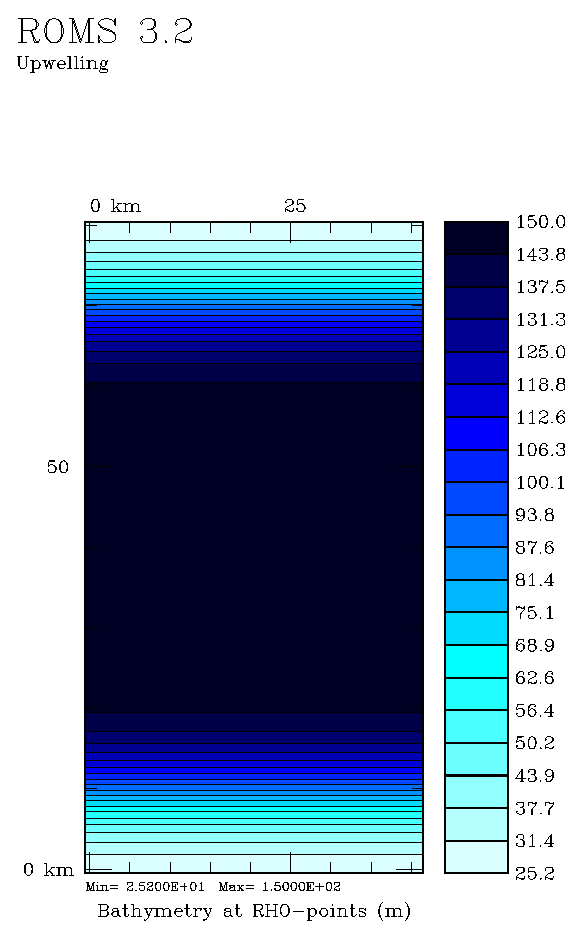
\includegraphics{pics/up1}
\end{picture}
\caption{The upwelling/downwelling bathymetry.}
\label{fsm1}
\end{figure}

\begin{figure}
\setlength{\unitlength}{10mm}
\begin{picture}(0,16)(0,0)
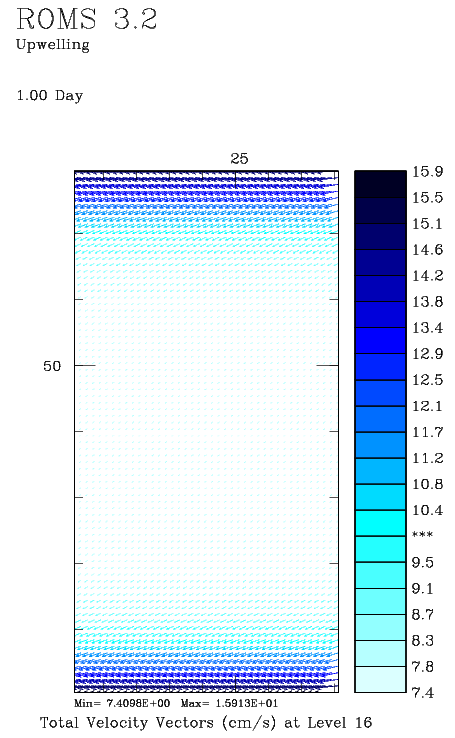
\includegraphics{pics/up2}
  \end{picture}
\caption{Surface velocities after one day, showing the flow to the
left of the wind (southern hemisphere).}
\end{figure}

\begin{figure}
\setlength{\unitlength}{10mm}
\begin{picture}(0,16)(0,0)
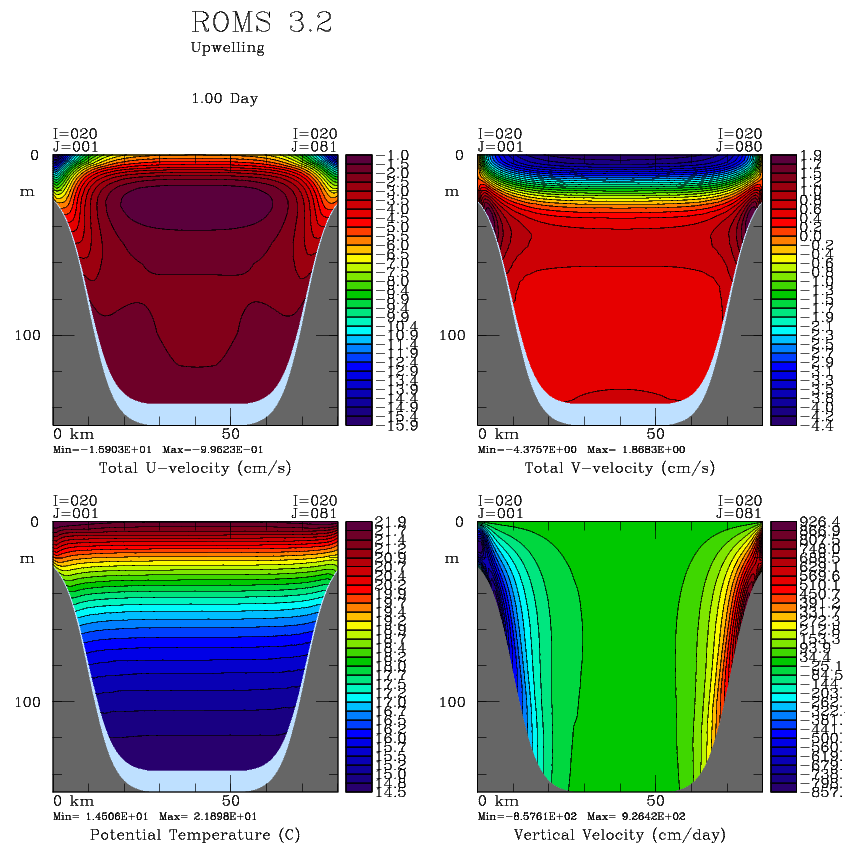
\includegraphics{pics/up3}
  \end{picture}
\caption{Constant $\xi$ slices of the $u, v, T$ and $w$ fields
at day 1.}
\end{figure}

\begin{figure}
\setlength{\unitlength}{10mm}
\begin{picture}(0,16)(0,0)
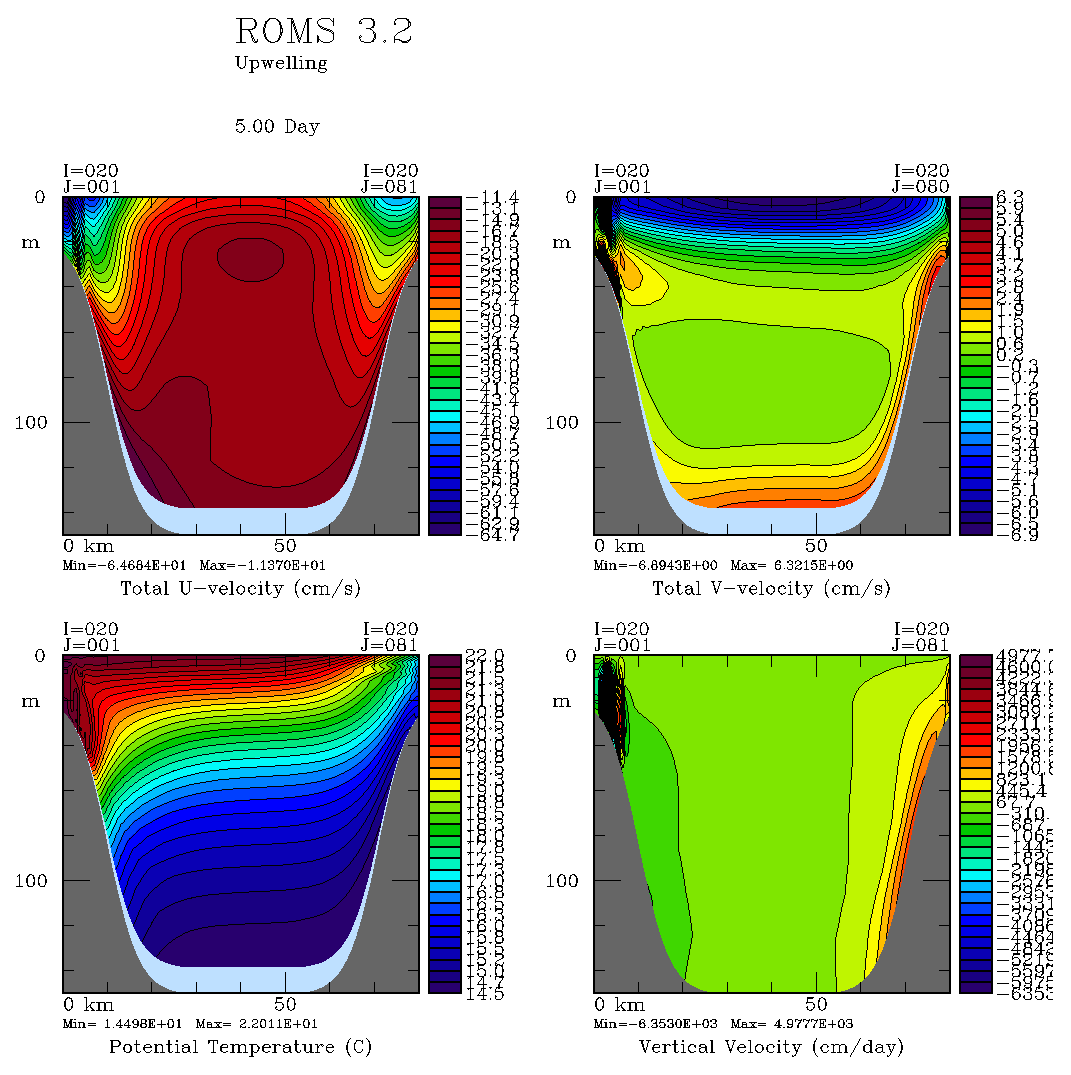
\includegraphics{pics/up4}
  \end{picture}
\caption{Constant $\xi$ slices of the $u, v, T$, and $w$ fields
at day 5.}
\label{fsm2}
\end{figure}

\subsection{Northeast Pacific example}
\label{NEP}
The upwelling/downwelling examples is one in which all the start-up
fields are defined analytically.  The other extreme is one in which
everything is read from files, as in our North Atlantic simulations.

\subsubsection{\code{cppdefs.h}}
The C preprocessor variable \code{DAMEE\_B} has been introduced to
make sure that we can \code{\#define DAMEE\_B} and have a
consistent configuration of the model.  This is done in part within
\code{cppdefs.h} by
\begin{verbatim}
                :
       # if defined DAMEE_B || defined DAMEE_S
       #define UV_ADV
       #define UV_GSCHEME
       #undef  UV_VIS2
       #undef  UV_VIS4
       #define UV_PRS
       #define UV_COR
       #undef  MIX_GP_UV
       #define TS_ADV
       #define TS_GSCHEME
       #undef  TS_DIF2
       #undef  TS_DIF4
       #undef  MIX_GP_TS
       #undef  SMOLARKIEWICZ
       #define NONLIN_EOS
       #define SALINITY
       #undef  DIAGNOSTIC
       #define QCORRECTION
       #define CURVGRID
       #define AVERAGES
       #undef  STATIONS
       #undef  OBC_EAST
       #undef  OBC_WEST
       #define OBC_NORTH
       #define OBC_SOUTH
       #undef  EW_PERIODIC
       #undef  NS_PERIODIC
       #undef  INFLOW
       #define OBC_TPRESCRIBE
       #define MASKING
       #define TIME_AVG
       #define BODYFORCE
       #undef  BVF_MIXING
       #undef  PP_MIXING
       #define LMD_MIXING
       #define LMD_RIMIX
       #define LMD_CONVEC
       #undef  LMD_DDMIX
       #define LMD_KPP
       #define CLIMATOLOGY
       #define NUDGING
       #define ANA_MEANRHO
       #undef  ANA_SMFLUX
       #undef  ANA_SSFLUX
       #undef  ANA_STFLUX
       #undef  ANA_SRFLUX
       #define ANA_BSFLUX
       #define ANA_BTFLUX
       #undef  ANA_V2DBC
       # endif /* DAMEE_B || DAMEE_S */
\end{verbatim}
Here, we have declared that we want a closed basin (not periodic),
masking, salinity, and the non-linear equation of state.  We want
Laplacian viscosity and diffusion along constant $z$-surfaces and the
full non-linear, curvilinear momentum equations.

We also added the DAMEE flags to \code{checkdefs.F}:
\begin{verbatim}
      #ifdef DAMEE_B
            write(stdout,20) 'DAMEE_B',
           &                 'North Atlantic DAMEE Big Domain Application.'
            is=lenstr(Coptions)+1
            Coptions(is:is+9)=' DAMEE_B,'
            iexample=iexample+1
      #endif /* DAMEE_B */
      #ifdef DAMEE_S
            write(stdout,20) 'DAMEE_S',
           &                 'North Atlantic DAMEE Small Domain Application.'
            is=lenstr(Coptions)+1
            Coptions(is:is+9)=' DAMEE_S,'
            iexample=iexample+1
      #endif /* DAMEE_S */
\end{verbatim}

\subsubsection{Model domain}
A large number of horizontal grid points was chosen to resolve the
domain at less than one degree.  Values for \code{L}, \code{M},
\code{N}, and \code{NT} are:
\begin{tabbing}
  Gnus Armadillos Pelicans \= \kill
  \> \code{L} = 129 \\
  \> \code{M} = 129 \\
  \> \code{N} = 20 \\
  \> \code{NT} = 2.
\end{tabbing}

\subsubsection{\code{gridpak}}
The grid has uniform spacing on a Mercator projection so that both
$\Delta x$ and $\Delta y$ get smaller as you get farther from the
equator.  The grid was chosen to go from 30$^\circ$ S to 65$^\circ$ N
and was generated with \code{sqgrid}.  We then found the latitude and
longitude values with \code{tolat} and interpolated the \code{etopo5}
bathymetry to the grid with \code{bathtub}.  The grid is shown in
Fig.\ \ref{fdg} and the unsmoothed bathymetry is shown in Fig.\
\ref{fdb1}.  It is clear that the unsmoothed bathymetry contains some
incredibly steep regions.  We have not pushed SCRUM to see what its
steepness limit is, but we also ran SPEM in this configuration and its
elliptic solver requires substantial smoothing at this resolution.
We were advised by Bernard Barnier to retain the shallow island
arc in the Caribbean.  We also had some bad experiences with shelves
that disappeared into the land mask, such as at Cape Hatteras and
the Iberian peninsula.  We filled in the Pacific and the Mediterranean
and did some unspeakable hacking to \code{bathsuds} to obtain the
bathymetry shown in Fig.\ \ref{fdb2}.  We then ran \code{sphere} to
obtain the values of $m$ and $n$ suitable for a spherical Earth and ran
Hernan Arango's mask editing tool \code{scrum\_mask}.

\begin{figure}
\setlength{\unitlength}{1cm}
  \begin{picture}(12,16)(-.72,0)
    \epsfbox{metafiles/dgrid.epsi}
  \end{picture}
\caption{The North Atlantic grid.}
\label{fdg}
\end{figure}

\begin{figure}
\setlength{\unitlength}{1cm}
  \begin{picture}(12,16)(.25,0)
    \epsfbox{metafiles/bath1.epsi}
  \end{picture}
\caption{The raw bathymetry from \code{etopo5}.}
\label{fdb1}
\end{figure}

\begin{figure}
\setlength{\unitlength}{1cm}
  \begin{picture}(12,16)(.25,0)
    \epsfbox{metafiles/bath2.epsi}
  \end{picture}
\caption{The smoothed North Atlantic bathymetry.}
\label{fdb2}
\end{figure}

\subsubsection{Initial conditions}
We would like the initial conditions to be a motionless fluid with
temperature and salinity fields from the Levitus 1994 February mean
climatology.  We prepared a NetCDF file with zero $u$, $v$ and $\zeta$
fields.  The $T$ and $S$ fields were interpolated from the Levitus
fields---we tried several different interpolation/extrapolation
techniques, including the \code{oa} program described in \S\ref{OA}.

An analytic function for the mean density was added to
\code{ana\_meanRHO} for this problem:
\begin{verbatim}
# elif defined DAMEE_B || defined DAMEE_S
         do k=1,N
           do j=0,M
             do i=0,L
               rhobar(i,j,k)=30.5-0.004*z_r(i,j,k)-
        &                         c4*exp(z_r(i,j,k)/2000.0)
             enddo
           enddo
         enddo
\end{verbatim}

\subsubsection{Boundary conditions}
The non-periodic option has already been chosen by not defining
\code{EW\_PERIODIC} or \code{NS\_PERIODIC} in \code{cppdefs.h}.
After trying a number of options, we ended up with walls to the north
and south with nudging regions (see below).

\subsubsection{Forcing}
The forcing is provided by surface momentum, heat and salt fluxes from
the COADS dataset.  We apply the heat flux correction
(\code{\#define} \code{QCORRECTION}), which is also provided in COADS.
We use the \code{oa} program to put the values onto the model grid for
each of the twelve monthly means.

\subsubsection{Climatology}
We used the same Levitus temperature and salinity fields for the
climatology as for the initial conditions.  The DAMEE problem was
specified to have nudging to the climatology at the northern and
southern boundaries, as well as at the Straits of Gibraltar.  We
edited \code{set\_nudgcof.F} to set the \code{nudgcof} array
accordingly.

\subsubsection{scrum.in}
We use an internal timestep of 2160 $s$ and an external timestep of 108
$s$.  The horizontal viscosity and diffusion is turned off (see above)
since the third-order upwind scheme is providing the smoothing.
The stretching parameters are $\theta = 5$, $b = .4$ and $h_c = 200 m$.

\subsubsection{Output}
The model writes out information to standard out:
\begin{verbatim}

 SCRUM input parameters:

    144000  ntimes      Number of timesteps to evolve 3-D equations.
   2160.00  dt          Timestep size (s) for 3-D equations.
        20  ndffast     Number of timesteps for 2-D equations between each DT.
         0  nrrec       Number of restart records to read from disk.
       400  nrst        Number of timesteps between storage of restart fields.
      1200  nwrt        Number of timesteps between writing fields into
                        history file.
         1  ntsavg      Starting timestep for the accumulation of output
                        time-averaged data.
      1200  navg        Number of timesteps between writing of time-averaged
                        data into averages file.
         1  ninfo       Number of timesteps between print of information 
                        to standard output.
         T  ldefhis     Switch to create a new history NetCDF file.
         T  lcycle      Switch to recycle time-records in restart NetCDF file.
 1.000E-05  Akt_bak(1)  Background vertical mixing coefficient (m^2/s)
                        for tracer 1.
 1.000E-05  Akt_bak(2)  Background vertical mixing coefficient (m^2/s)
                        for tracer 2.
 1.000E-04  Akv_back    Background vertical mixing coefficient (m^2/s)
                        for momentum.
 3.000E-04  rdrg        Linear bottom drag coefficient (m/s).
 0.000E+00  rdrg2       Quadratic bottom drag coefficient.
        18  levsfrc     Deepest level to apply surface stress as a body force.
         1  levbfrc     Shallowest level to apply bottom stress as a body force.
 5.000E+00  theta_s     S-coordinate surface control parameter.
 4.000E-01  theta_b     S-coordinate bottom  control parameter.
  200.0000  Tcline      S-coordinate surface/bottom layer width (m) used
                        in vertical coordinate stretching.
 1000.0000  rho0        Mean density (kg/m^3) used in Boussinesq approximation.
   30.0000  dstart      Time stamp assigned to model initialization (days).
    0.0000  T0          Background potential temperature (Celsius) constant.
    0.0000  S0          Background salinity (PSU) constant.
      1.00  gamma2      Slipperiness variable: free-slip (1.0) or 
                                               no-slip (-1.0).
         T  wall1       Boundary for side 1 (i=1): wall/open (T/F).
         T  wall2       Boundary for side 2 (j=1): wall/open (T/F).
         T  wall3       Boundary for side 3 (i=L): wall/open (T/F).
         T  wall4       Boundary for side 4 (j=M): wall/open (T/F).
         T  wrtU        Write out 3D U-momentum component (T/F).
         T  wrtV        Write out 3D V-momentum component (T/F).
         T  wrtW        Write out W-momentum component (T/F).
         F  wrtO        Write out omega vertical velocity (T/F).
         T  wrtUBAR     Write out 2D U-momentum component (T/F).
         T  wrtVBAR     Write out 2D V-momentum component (T/F).
         T  wrtZ        Write out free-surface (T/F).
         T  wrtT(1)     Write out tracer 1 (T/F).
         T  wrtT(2)     Write out tracer 2 (T/F).
         F  wrtRHO      Write out density anomaly (T/F).
         T  wrtAKV      Write out vertical viscosity coefficient (T/F).
         T  wrtAKT      Write out vertical T-diffusion coefficient (T/F).
         T  wrtAKS      Write out vertical S-diffusion coefficient (T/F).
         T  wrtHBL      Write out depth of mixed layer (T/F).

Scrum 3.0 - North Atlantic Damee 4: Annual Levitus 0.75 resolution
       


 Output/Input Files:

            Output Restart File:  scrum_rst.nc
           Output Averages File:  scrum_avg.nc
                Input Grid File:  damee_grid_4.nc
             Input Initial File:  damee_lev_4feb.nc
             Input Forcing File:  frc_coads_4.nc
         Input Climatology File:  damee_clm_4L.nc
         Input/Output USER File:  /dev/null

 Activated C-preprocessing Options:

  ANA_BSFLUX       Analytical kinematic bottom salt flux.
  ANA_BTFLUX       Analytical kinematic bottom heat flux.
  ANA_MEANRHO      Analytical mean density anomaly.
  AVERAGES         Writing out time-averaged fields.
  BODYFORCE        Momentum stresses as body-forces.
  CURVGRID         Orthogonal curvilinear grid.
  DAMEE_B          North Atlantic DAMEE Big Domain Application.
  DBLEPREC         Double precision arithmetic.
  LMD_CONVEC       LMD convective mixing due to shear instability.
  LMD_MIXING       Large/McWilliams/Doney interior mixing.
  LMD_KPP          Large/McWilliams/Doney boundary layer mixing.
  LMD_RIMIX        LMD diffusivity due to shear instability.
  MASKING          Land/Sea masking.
  MIX_GP_TS        Mixing of tracers along geopotential surfaces.
  MIX_GP_UV        Mixing of momentum along geopotential surfaces.
  NONLIN_EOS       Non-linear Equation of State for seawater.
  NUDGING          Nudging toward climatology.
  OBC_NORTH        Open North boundary edge.
  OBC_SOUTH        Open South boundary edge.
  OBC_TREDUCED     Tracers, boundary reduced physics condition.
  QCORRECTION      Surface net heat flux correction.
  SALINITY         Using salinity.
  SOLVE2D          Solving 2D Primitive Equations.
  SOLVE3D          Solving 3D Primitive Equations.
  TCLIMATOLOGY     Processing tracer climatology data.
  TIME_AVG         Time averaging over two short timestep cycles.
  TNUDGING         Nudging toward tracer climatology.
  TS_ADV           Advection of tracers.
  TS_GSCHEME       Shchepetkin-McWilliams G-Scheme Advection of tracer.
  UV_ADV           Advection of momentum.
  UV_COR           Coriolis term.
  UV_GSCHEME       Shchepetkin-McWilliams G-Scheme Advection of momentum.
  UV_PRS           Hydrostatic pressure gradient term.

 Vertical S-coordinate System: 

   level    S-coord   at hmin    over slope    at hmax

   20        0.00        0.00        0.00        0.00
   19       -0.05      -10.00      -20.03      -30.05
   18       -0.10      -20.00      -43.30      -66.60
   17       -0.15      -30.00      -71.92     -113.84
   16       -0.20      -40.00     -108.94     -177.89
   15       -0.25      -50.00     -158.64     -267.27
   14       -0.30      -60.00     -226.50     -393.01
   13       -0.35      -70.00     -318.60     -567.19
   12       -0.40      -80.00     -439.47     -798.94
   11       -0.45      -90.00     -588.95    -1087.90
   10       -0.50     -100.00     -759.64    -1419.28
    9       -0.55     -110.00     -938.48    -1766.95
    8       -0.60     -120.00    -1112.90    -2105.81
    7       -0.65     -130.00    -1277.09    -2424.19
    6       -0.70     -140.00    -1433.59    -2727.18
    5       -0.75     -150.00    -1591.00    -3032.00
    4       -0.80     -160.00    -1761.00    -3361.99
    3       -0.85     -170.00    -1956.64    -3743.28
    2       -0.90     -180.00    -2192.17    -4204.35
    1       -0.95     -190.00    -2483.64    -4777.28
    0       -1.00     -200.00    -2850.00    -5500.00

      GET_INITIAL - Processing initial conditions  for time = 0.0000E+00
      GET_SRFLUX  - Read solar shortwave radiation for time =    345.0
      GET_STFLUX  - Read surface flux of tracer 01 for time =    345.0
      GET_STFLUX  - Read surface flux of tracer 02 for time =    345.0
      GET_SMFLUX  - Read surface momentum stresses for time =    345.0
      GET_TCLIMA  - Read climatology of tracer  01 for time = 0.0000E+00
      GET_TCLIMA  - Read climatology of tracer  02 for time = 0.0000E+00

 MAIN - started time-stepping SCRUM: 

      GET_SRFLUX  - Read solar shortwave radiation for time =    15.00
      GET_STFLUX  - Read surface flux of tracer 01 for time =    15.00
      GET_STFLUX  - Read surface flux of tracer 02 for time =    15.00
      GET_SMFLUX  - Read surface momentum stresses for time =    15.00
 
 Day =      0.025000  avgKE =  9.587033E-16  avgPE =  7.947536E-07
 Day =      0.050000  avgKE =  9.608381E-16  avgPE =  7.947534E-07
 Day =      0.075000  avgKE =  9.583708E-16  avgPE =  7.947537E-07
                     :
\end{verbatim}
It also writes out NetCDF files for restart, history, and monthly
averages.  Plots can be made from all three of these files; an example
plot is shown in Fig.\ \ref{fdz1}.

\begin{figure}
\setlength{\unitlength}{1cm}
  \begin{picture}(12,16)(-.8,0)
    \epsfbox{metafiles/damee1.epsi}
  \end{picture}
\caption{The annual mean surface elevation for year 10.}
\label{fdz1}
\end{figure}
